% Chapter 5: Results

\chapter{Resultados} % Main chapter title

\label{Chapter5} % Reference

%-------------------------------------------------------------------------------

\section{Ejemplos de uso de la aplicación}

%En esta sección se va a poner un ejemplo de como un usuario utilizaría la aplicación ya descargada en su terminal móvil.
Esta sección muestra un ejemplo de uso completo de la aplicación, pasando por los prerrequisitos, el cifrado de un fichero y la descarga de un mensaje.

\begin{figure}[!htb]
  \centering
  
\includegraphics[scale=0.2]{Figures/launcher}
  \decoRule
  \caption[Shatter (Icono)]{Icono de la aplicación Shatter}
  \label{fig:launcher}
\end{figure}

\subsection{Prerrequisitos}

Al tratarse de una aplicación Android, es necesario el uso de un dispositivo que utilice el Sistema Operativo Android (Véase~\ref{Android}), específicamente la versión 6 (Marshmallow) o una superior.

También es necesario dar permisos de escritura en el almacenamiento del dispositivo, ya que la aplicación realiza operaciones de escritura y lectura.

\subsection{Añadir contactos}

Al abrir la aplicación por primera vez se genera un par de claves asimétricas, una pública y otra privada. En la pantalla principal, al no disponer de ningún contacto, solo se puede ver un campo de texto, un botón para seleccionar un fichero y un botón para añadir usuarios. (Figura~\ref{fig:home})

\begin{figure}[!htb]
  \centering
  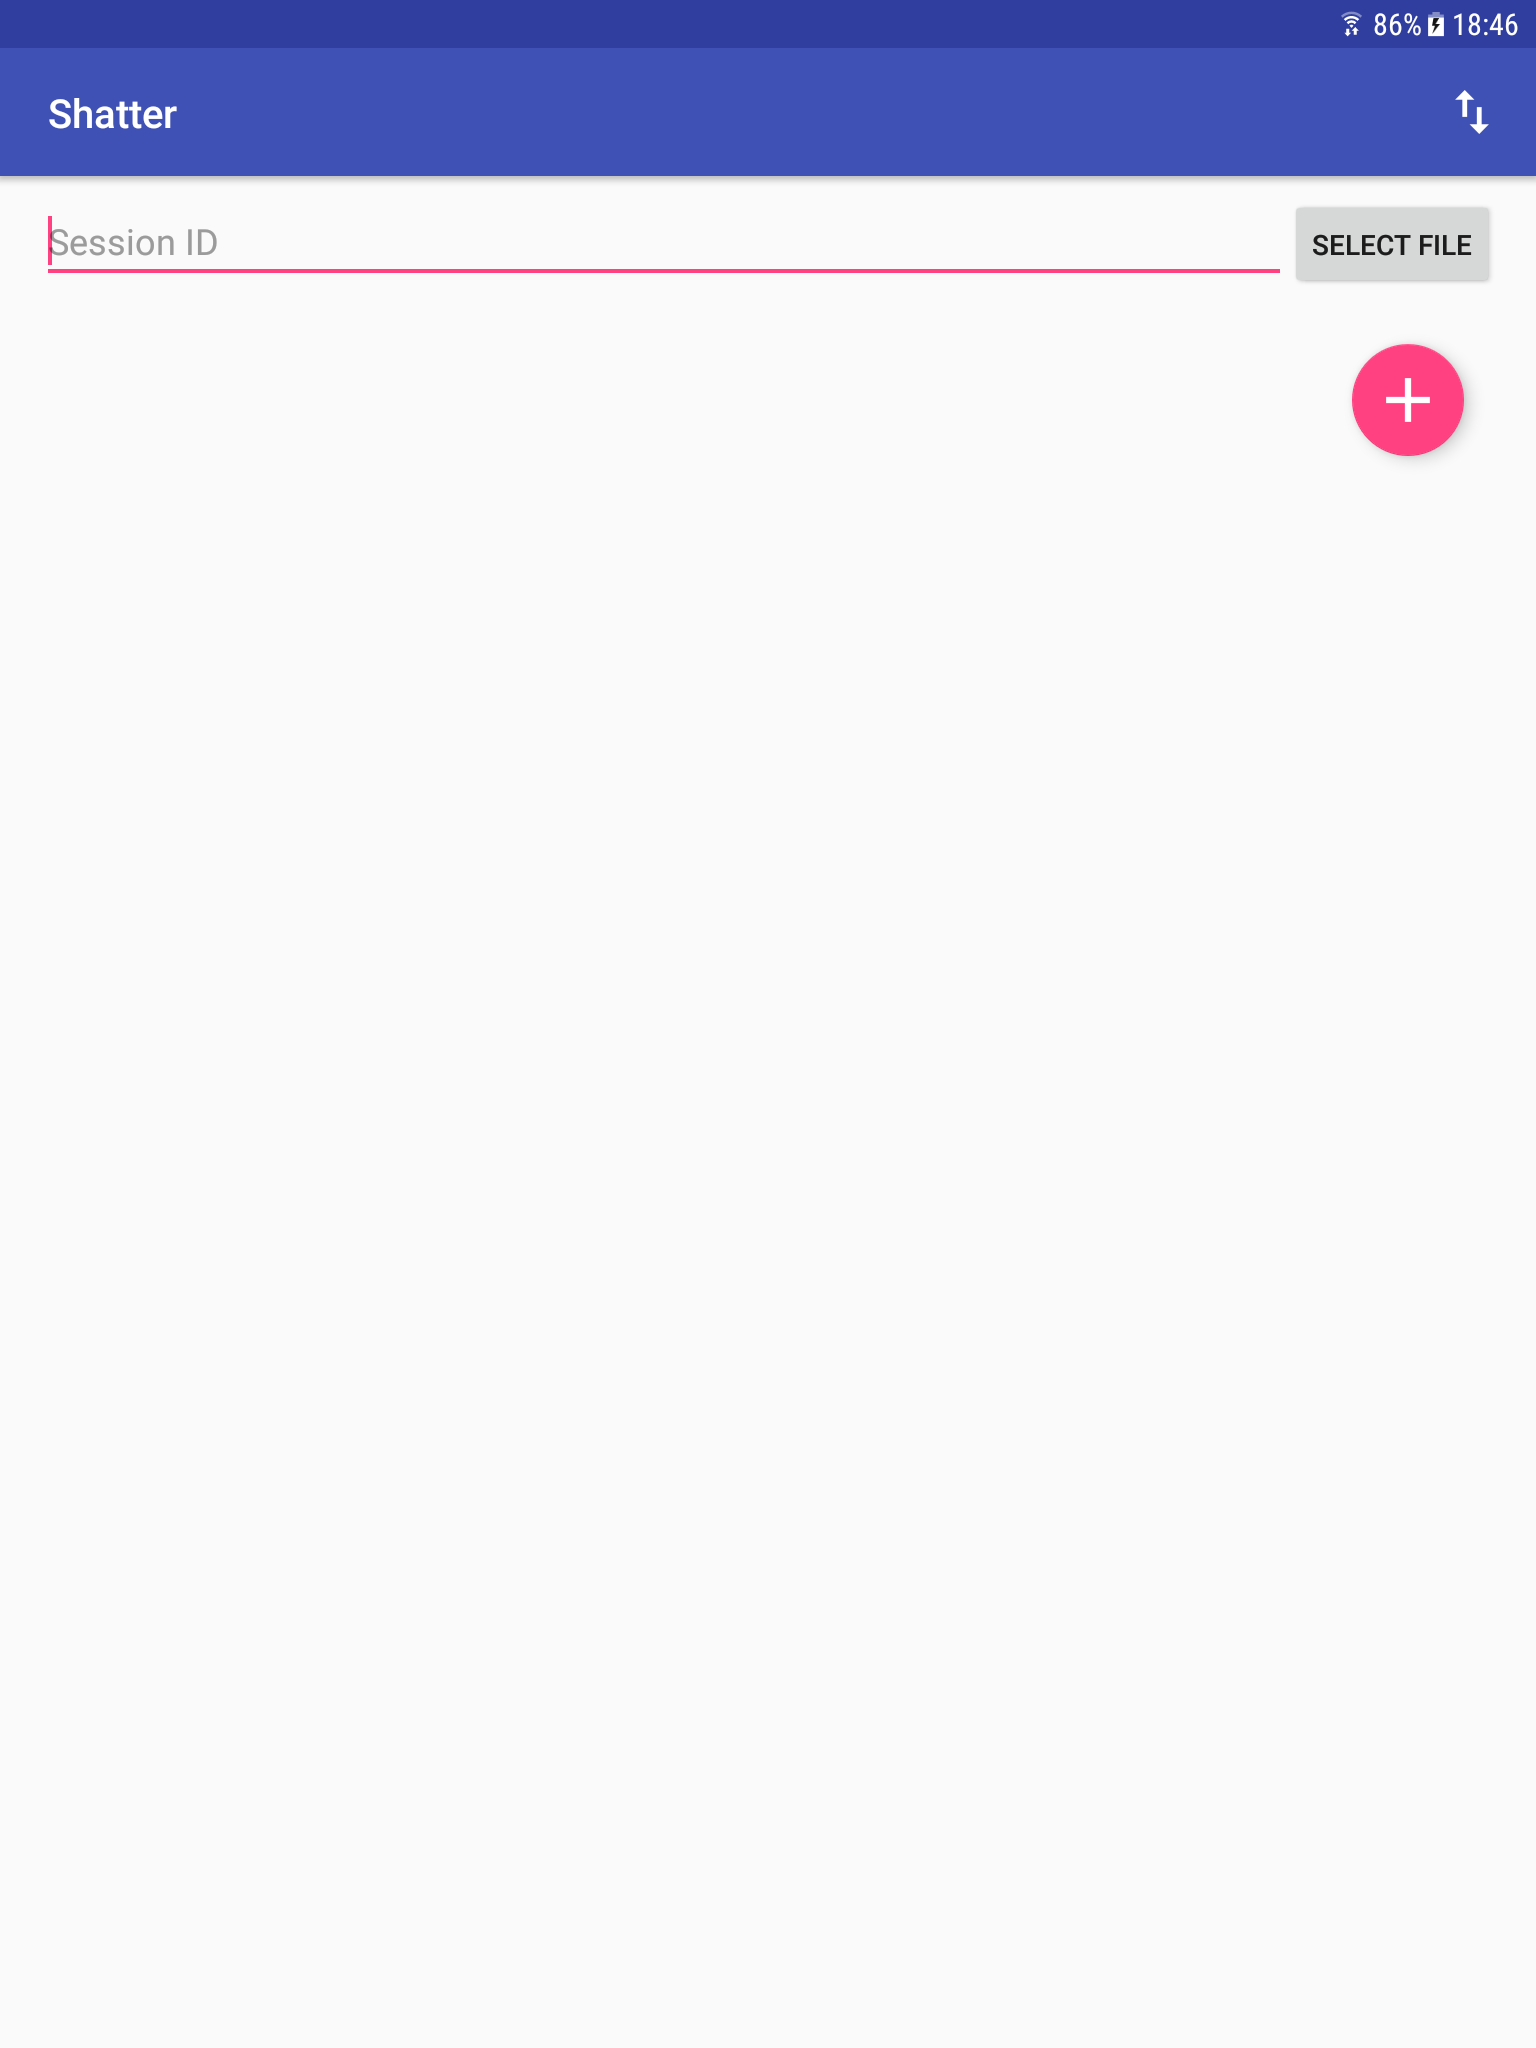
\includegraphics[scale=0.4]{Figures/home}
  \decoRule
  \caption[Shatter (Home)]{Pantalla principal de la aplicación}
  \label{fig:home}
\end{figure}

El primer objetivo es añadir algún usuario a la lista de contactos. Lo primero que hay que hacer es exportar la clave pública previamente generada haciendo uso del icono que se encuentra en la barra superior de la pantalla principal. (Figura~\ref{fig:export})

\begin{figure}[!htb]
  \centering
  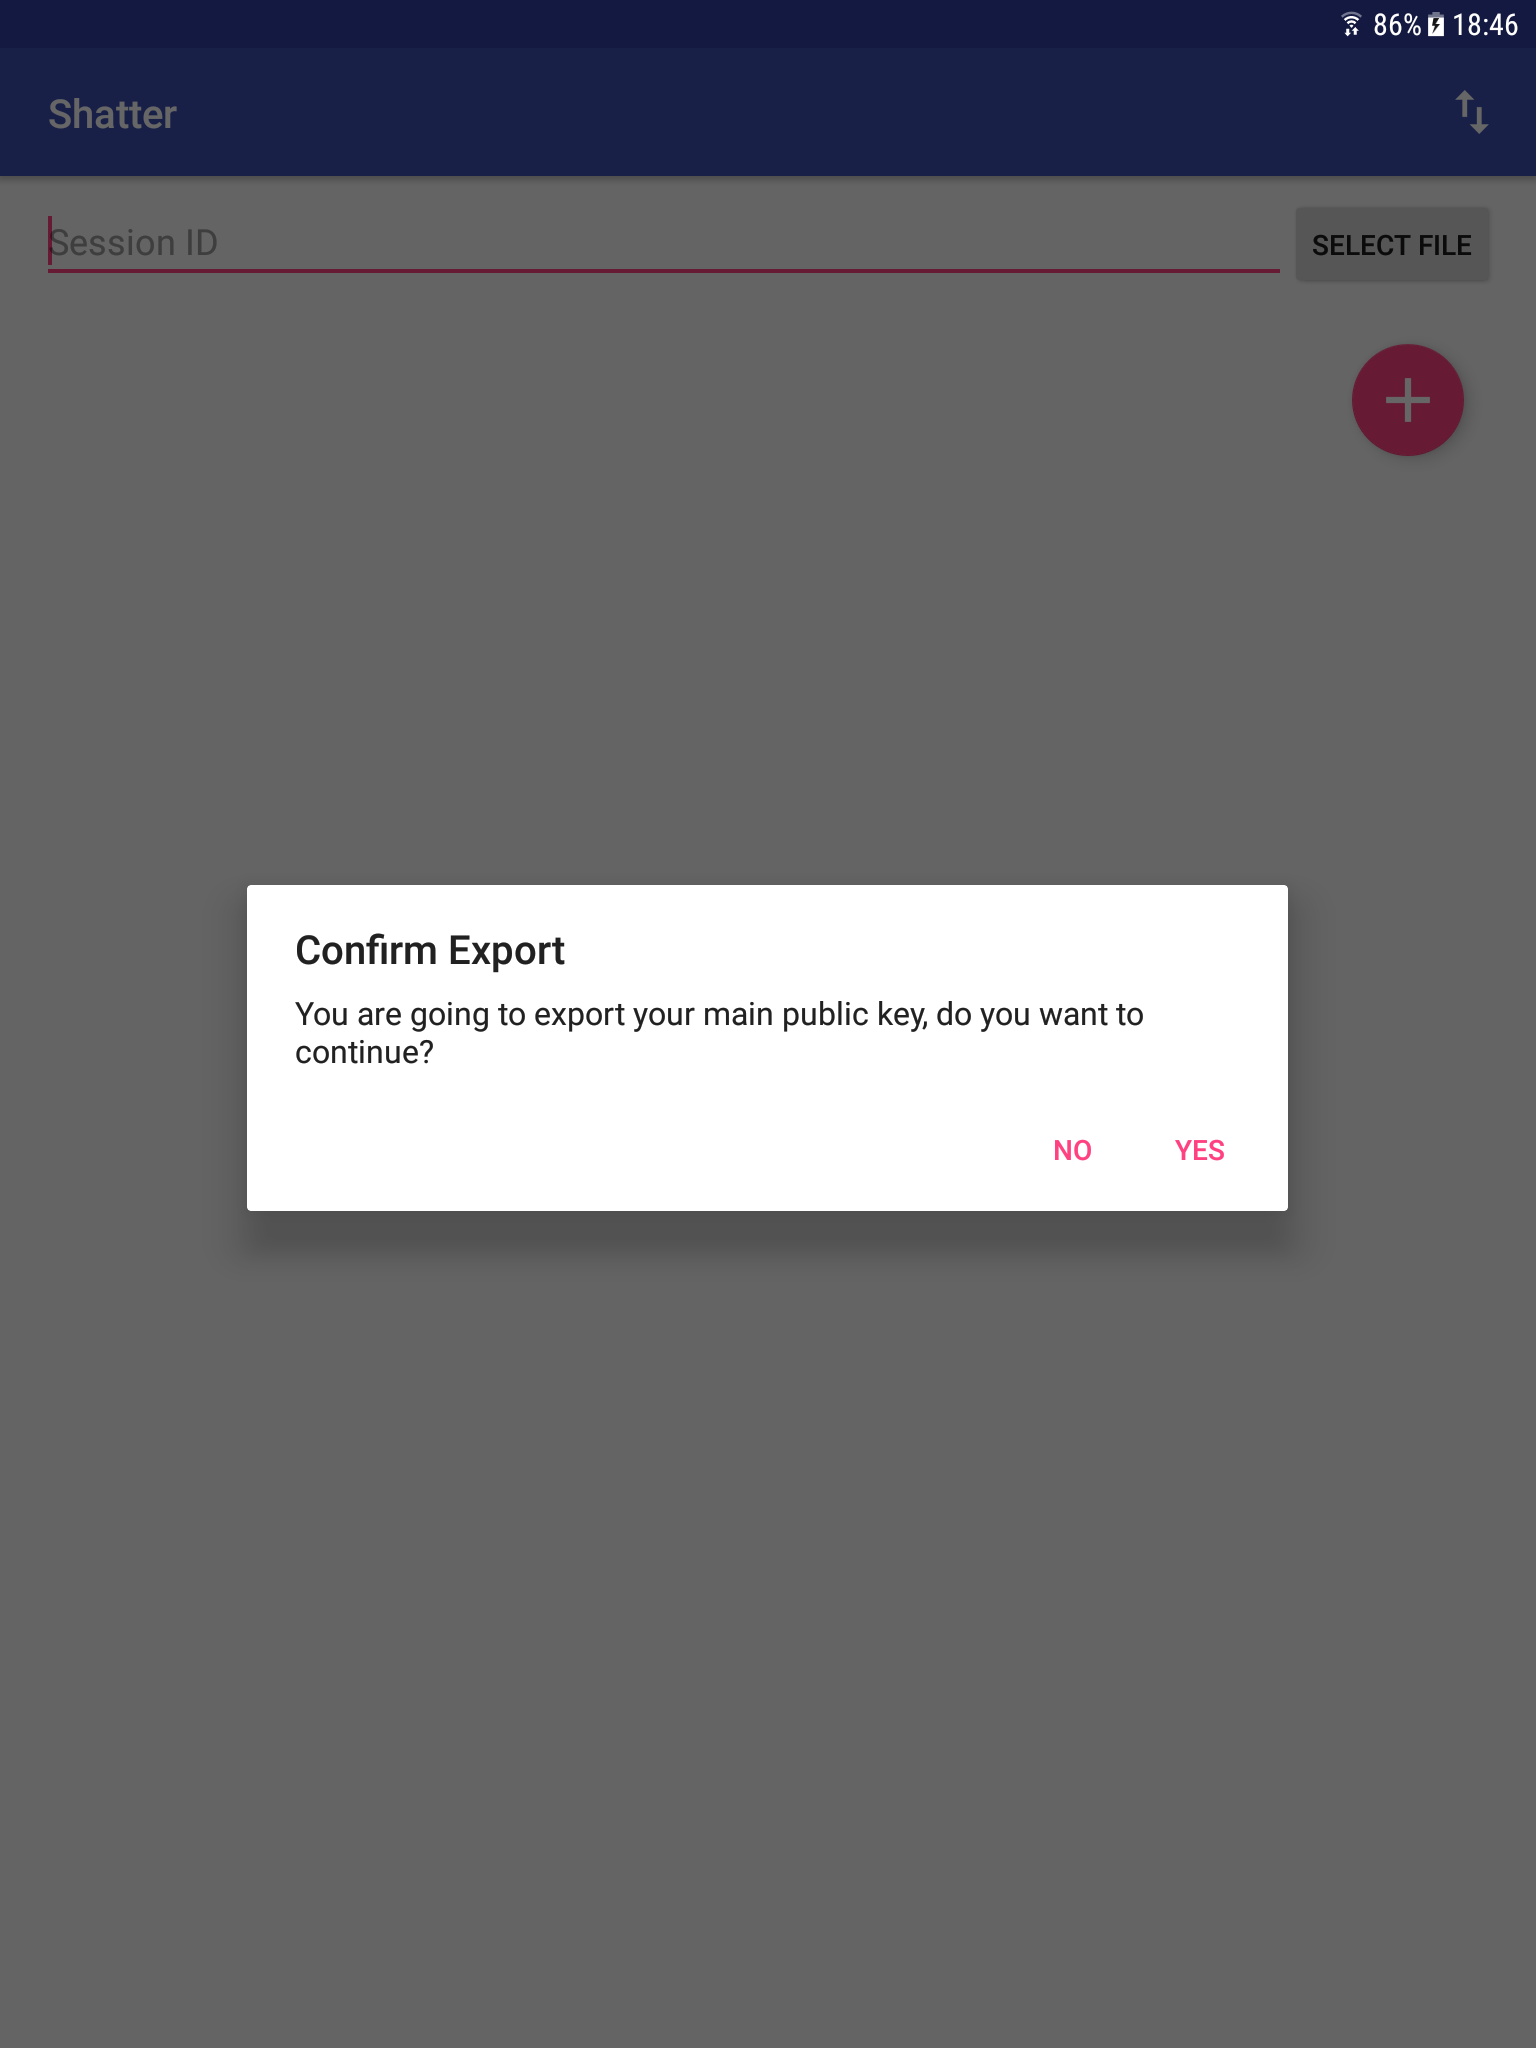
\includegraphics[scale=0.4]{Figures/export}
  \decoRule
  \caption[Shatter (Exportar clave pública)]{Mensaje de advertencia al exportar la clave pública}
  \label{fig:export}
\end{figure}

Al confirmar, se genera un certificado el cual contiene la clave pública antes generada en la ruta \path{Shatter/certs/main.crt}. \footnote{El directorio principal de la aplicación se encuentra en el almacenamiento externo del terminal y es accesible mediante un explorador de archivos.}

Para añadir a un contacto se dispone de un botón en la esquina inferior derecha de la pantalla principal, el cual abre una nueva pantalla en la que se puede especificar un alias (nombre de usuario) y un certificado con la clave pública del nuevo usuario. (Figura~\ref{fig:import})

\begin{figure}[!htb]
  \centering
  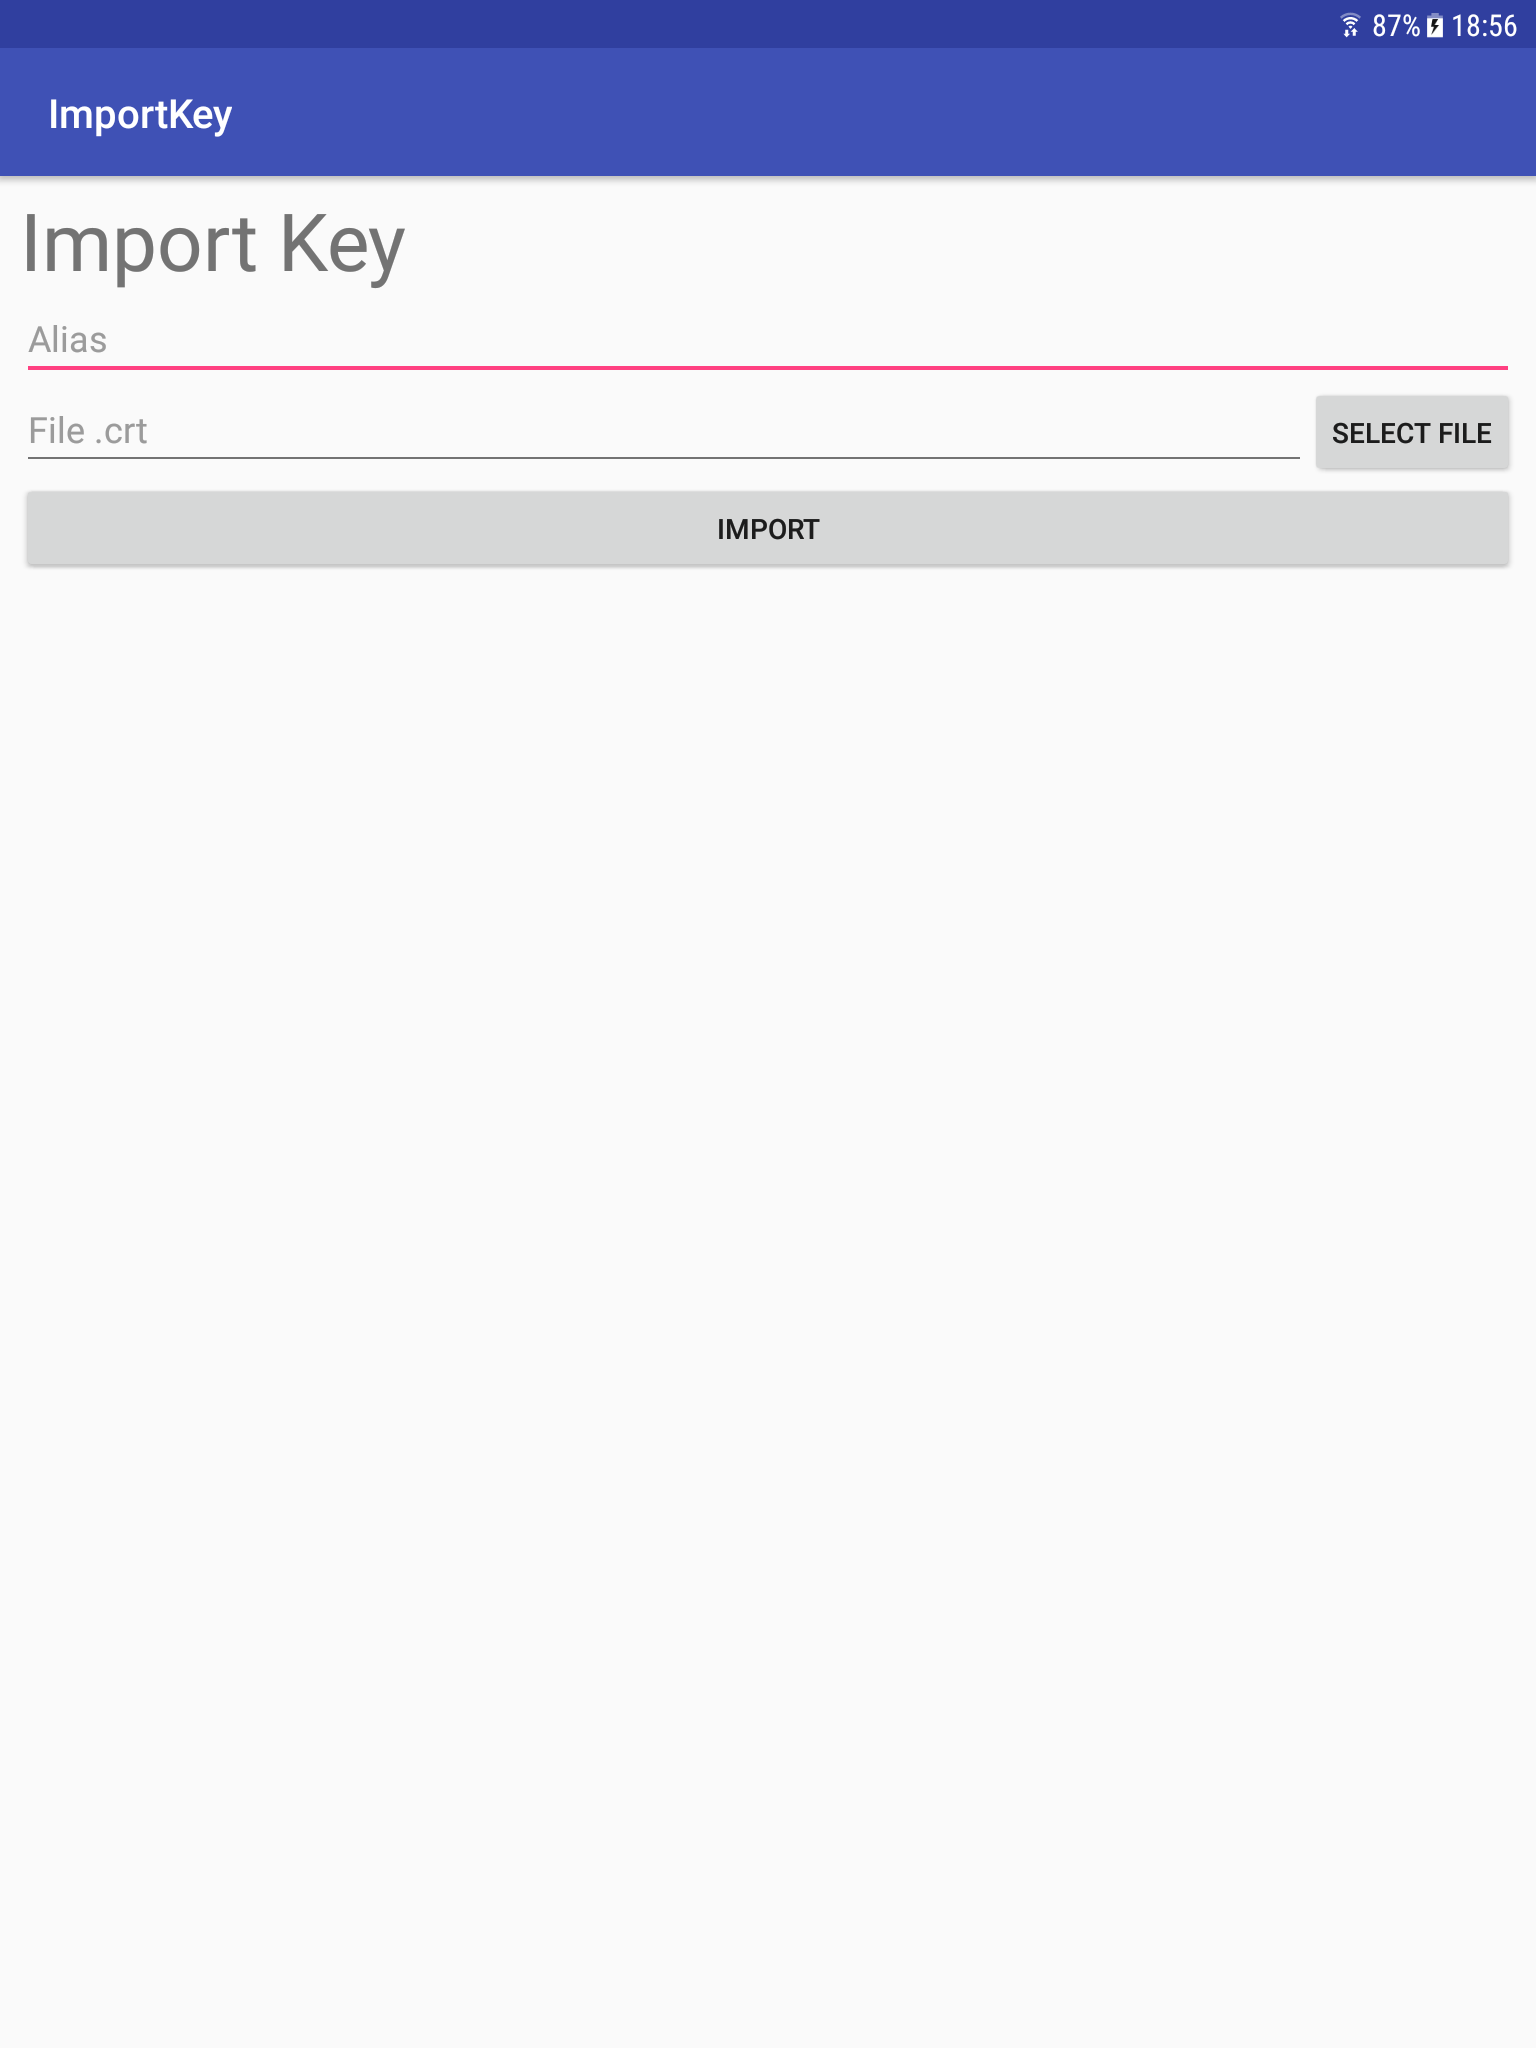
\includegraphics[scale=0.4]{Figures/import}
  \decoRule
  \caption[Shatter (Importar clave pública)]{Pantalla para importar la clave pública de un nuevo usuario}
  \label{fig:import}
\end{figure}

%De la misma manera, el nuevo contacto debe importar el certificado antes generado para poder llevar a cabo comunicaciones seguras.

Una vez el nuevo usuario se ha importado, la pantalla principal se actualiza y muestra el alias que tiene asignado, junto a unos botones con los que se puede operar con su clave pública. (Figura~\ref{fig:home_2})

\begin{figure}[!htb]
  \centering
  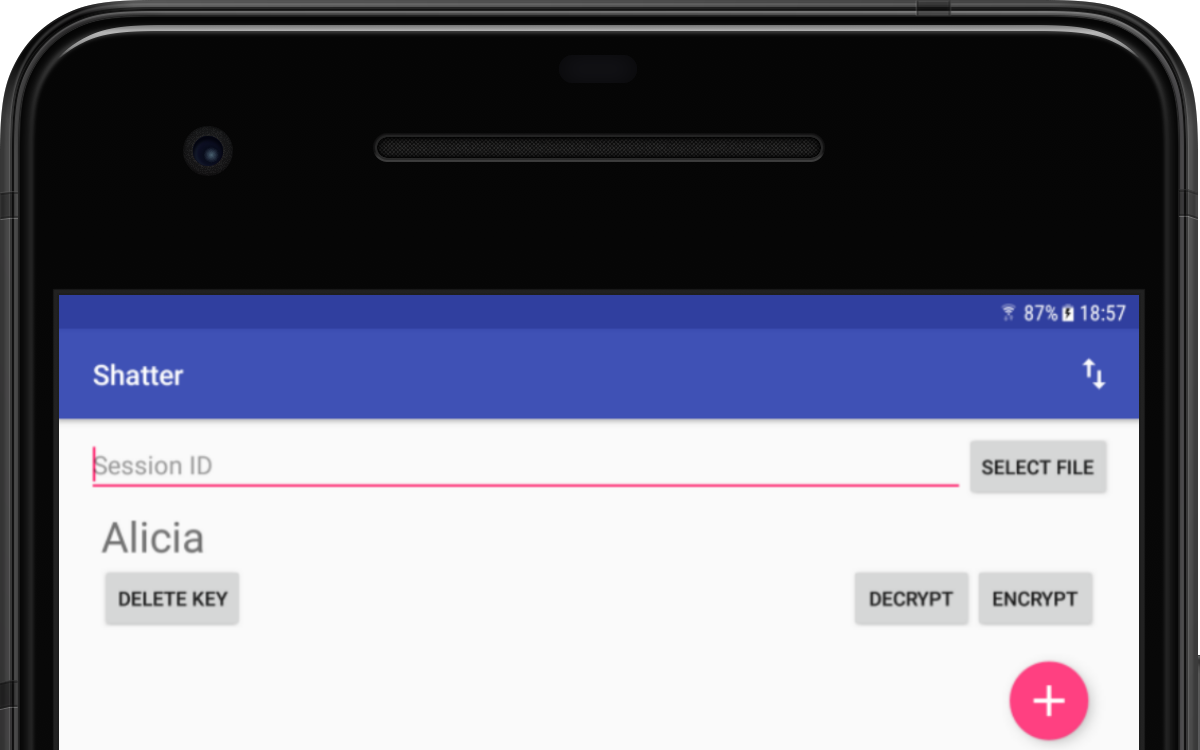
\includegraphics[scale=0.4]{Figures/home_2}
  \decoRule
  \caption[Shatter (Pantalla principal con usuarios)]{Pantalla principal de la aplicación con usuarios añadidos}
  \label{fig:home_2}
\end{figure}

\subsection{Cifrado y envío}

Para enviar un mensaje a un contacto, se debe utilizar el botón \keyword{\emph{Select File}}, el cual abre una nueva pantalla para elegir un fichero (Figura~\ref{fig:file_picker}). El selector de ficheros pone en el campo de texto de la pantalla principal el path absoluto del fichero seleccionado (también se puede escribir a mano), y ya solo queda tocar el botón \keyword{\emph{Encrypt}} del usuario al que vaya destinado el mensaje para que el fichero se fragmente y encripte. Si todo ha salido bien, se puede ver un mensaje en pantalla informando de ello, y en la ruta \path{Shatter/send/ID} se encuentran los fragmentos junto con la clave. (Figura~\ref{fig:encfiles})

\begin{figure}[!htb]
  \centering
  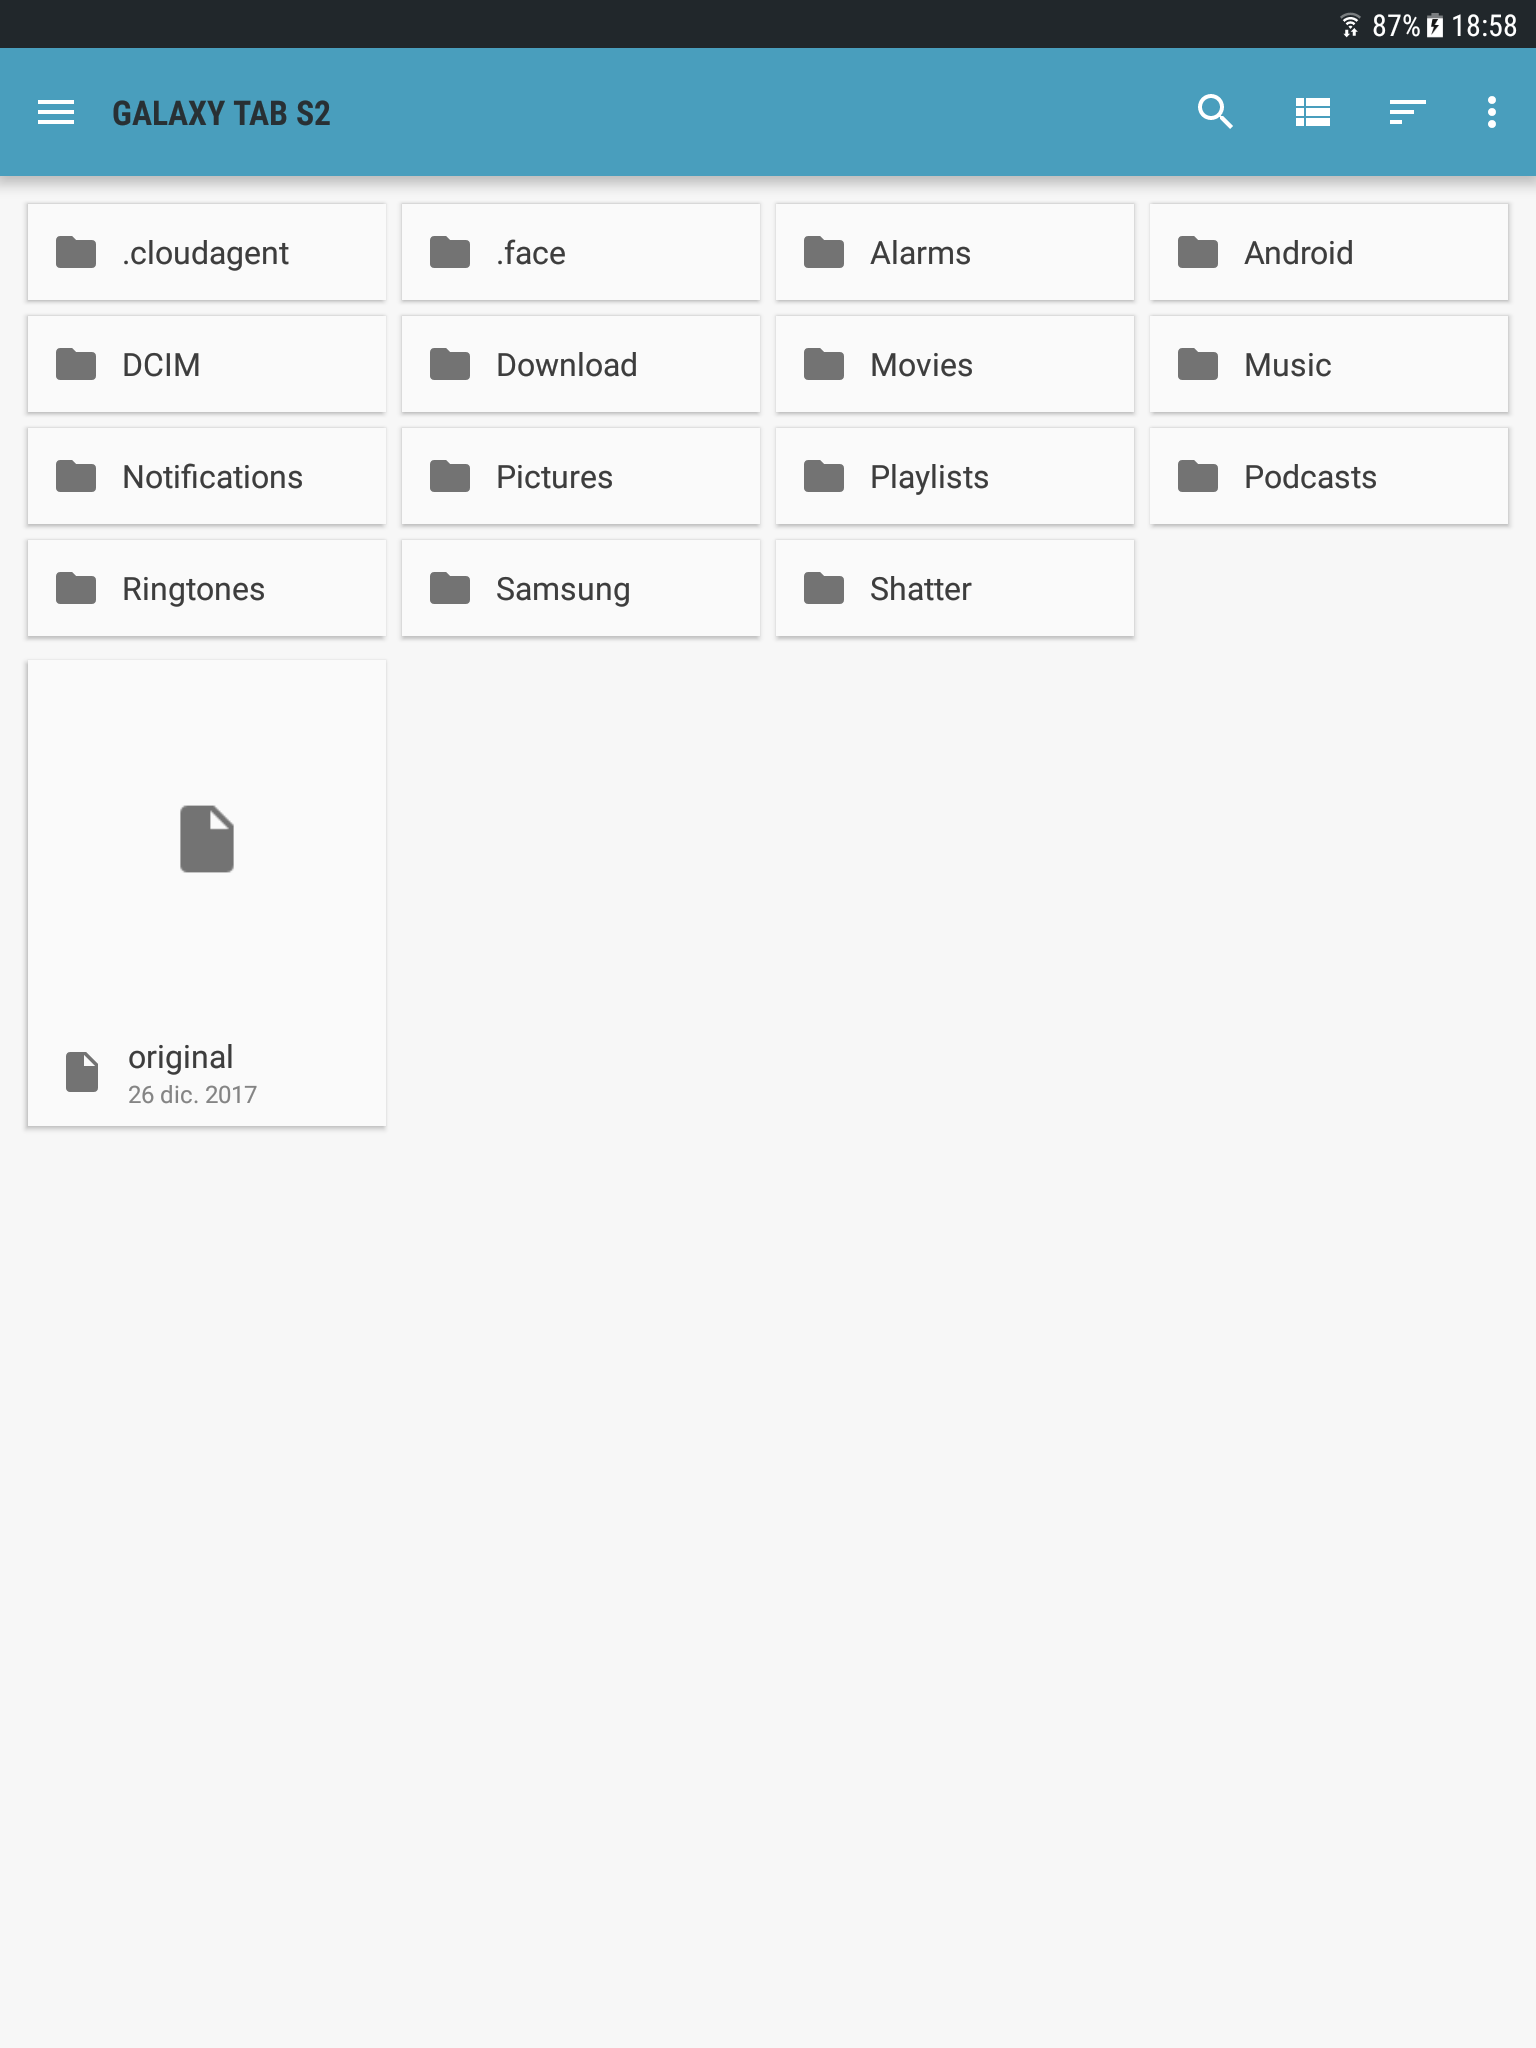
\includegraphics[scale=0.4]{Figures/file_picker}
  \decoRule
  \caption[Shatter (File Picker)]{Pantalla para seleccionar un fichero}
  \label{fig:file_picker}
\end{figure}

\begin{figure}[!htb]
  \centering
  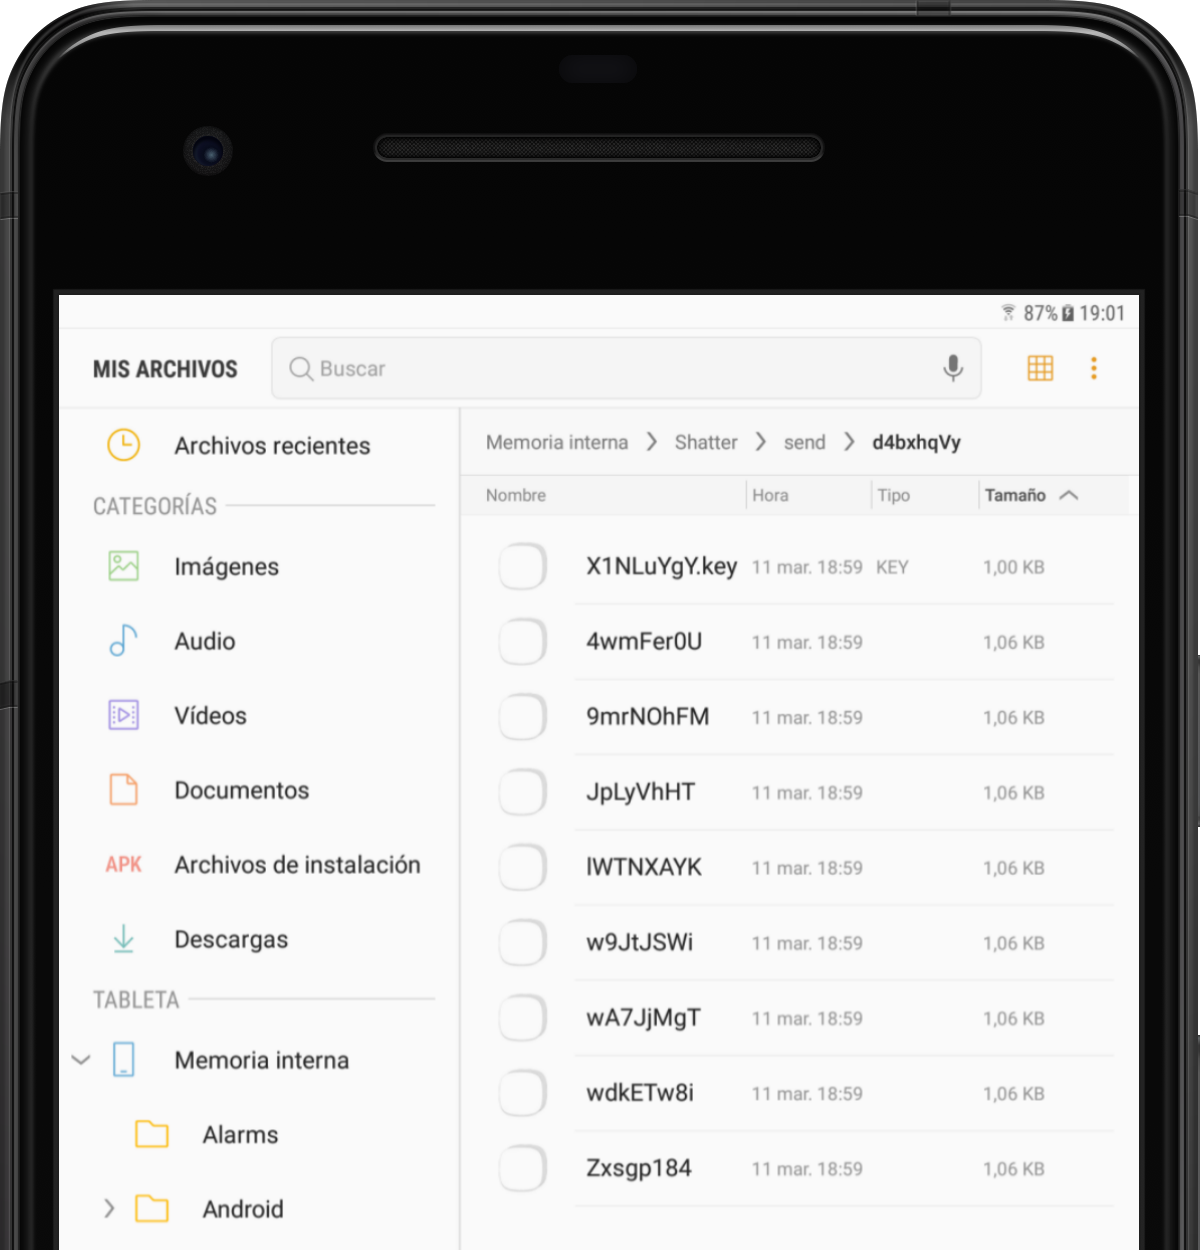
\includegraphics[scale=0.4]{Figures/encfiles}
  \decoRule
  \caption[Shatter (Mensaje fragmentado)]{Fragmentos de un mensaje junto a su clave}
  \label{fig:encfiles}
\end{figure}

El ID generado se debe comunicar al contacto al que vaya destinado, pero antes se debe subir el directorio que contiene los fragmentos al servidor haciendo uso del comando scp de Linux, por lo que se debe disponer de un usuario habilitado en la máquina que aloja el servidor. \footnote{En caso de estar encriptando el mismo mensaje para varios usuarios, se puede saber que ID corresponde a cada usuario mirando un registro que se encuentra en la ruta \path{Shatter/list.txt}}

\lstset{basicstyle=\ttfamily}
\begin{lstlisting}[language=bash]
  $ scp Shatter/send/ID server
\end{lstlisting}

\subsection{Descarga y descifrado}

Para descargar un mensaje de un contacto determinado, este debe comunicar de alguna manera el ID del mensaje, el cual se debe escribir en el campo de texto de la pantalla principal. A continuación se pulsa el botón \keyword{\emph{Decrypt}} asociado al alias del contacto.
%Si nuestro contacto quisiera descargarse el mensaje, escribirá el ID que le comunicamos antes en el campo de texto de la pantalla principal. Como sabe que el mensaje viene de nuestra parte, tocará el botón \emph{Decrypt} de nuestra clave pública.

Con esto, la aplicación pide al servidor un índice con todos los ficheros asociados a ese ID y descarga todos los que pueda en el directorio \path{Shatter/ID}. En caso de que algún fichero falte, informa de ello al usuario antes de proceder con el descifrado y rellena un registro indicando cuales son los fragmentos que faltan. (Figura~\ref{fig:miss})

\begin{figure}[!htb]
  \centering
  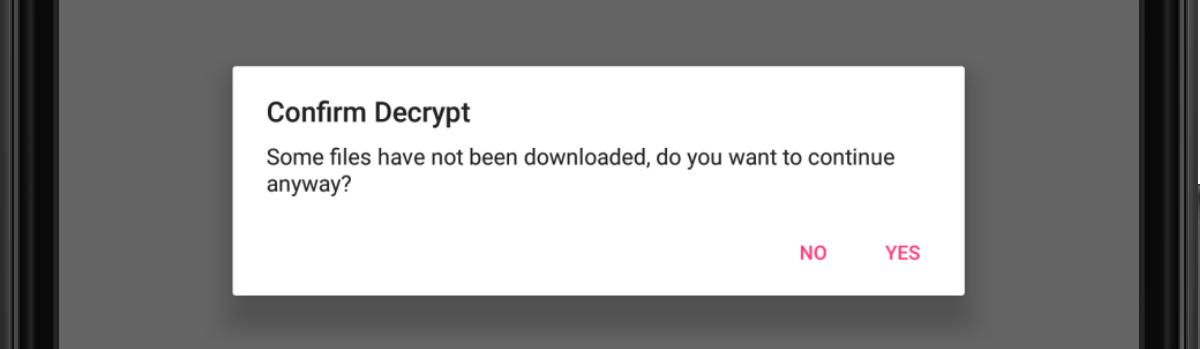
\includegraphics[scale=0.4]{Figures/miss}
  \decoRule
  \caption[Shatter (Faltan fragmentos)]{Mensaje advirtiendo de que algunos fragmentos no se han descargado}
  \label{fig:miss}
\end{figure}

Si todos los fragmentos y la clave son descargados exitosamente, la aplicación procede con el descifrado de los mismos. Durante el proceso se crean, en caso de ser necesario, ficheros de registro en los cuales se reflejan los problemas surgidos. En caso de no ocurrir ningún problema, el fichero original se recompone en la ruta \path{Shatter/ID/done/ID}. (Figura~\ref{fig:done})

\begin{figure}[!htb]
  \centering
  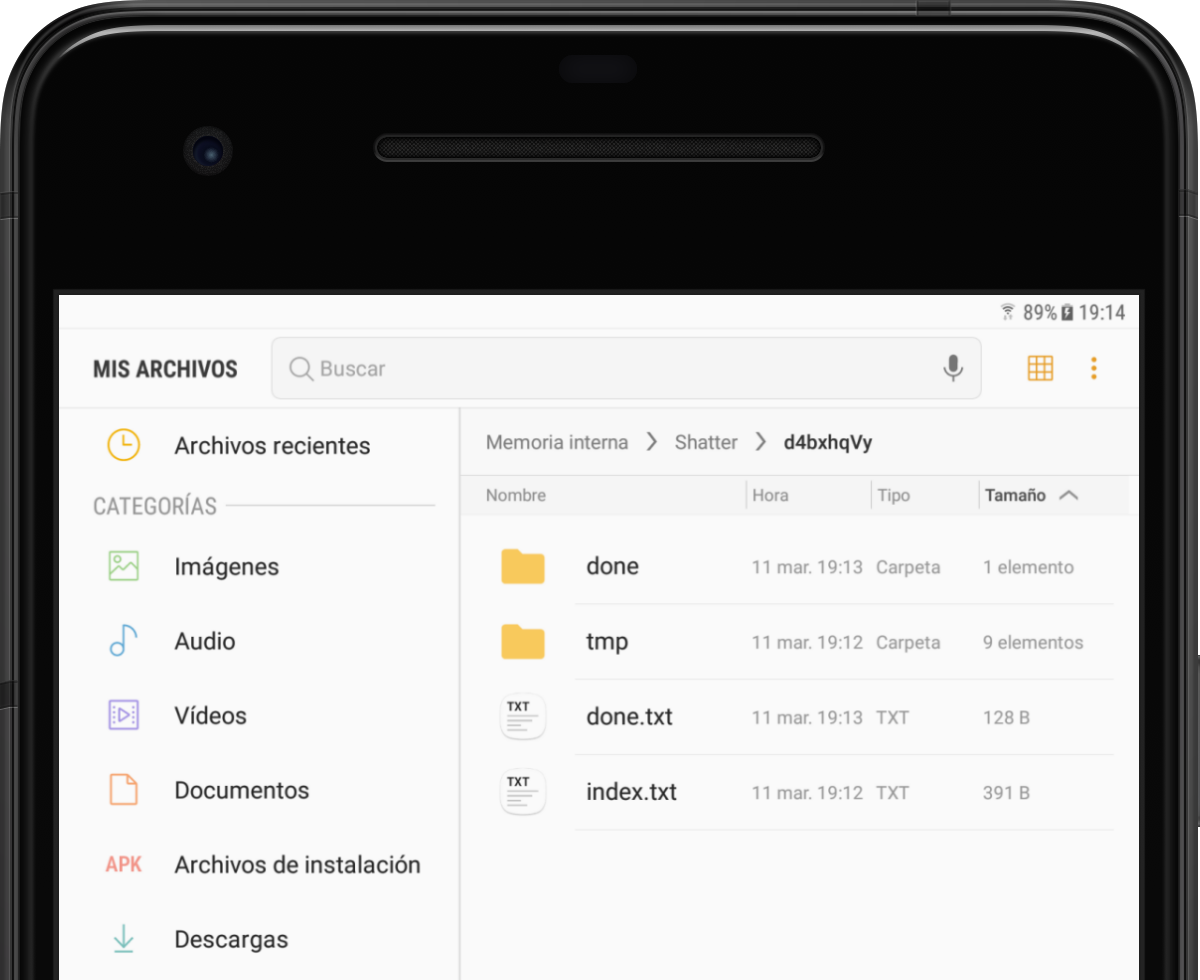
\includegraphics[scale=0.4]{Figures/done}
  \decoRule
  \caption[Shatter (Mensaje recibido)]{Directorio de un mensaje recibido}
  \label{fig:done}
\end{figure}

%-------------------------------------------------------------------------------

\section{Problemas encontrados}

A lo largo de la etapa que supuso el desarrollo de la aplicación, se han encontrado varios problemas que dificultaron la finalización del proyecto.

El mayor problema con el que se tuvo que lidiar es el no haber creado una parte portable que hiciera más fácil la migración a Android. Algunas librerías usadas cuando el proyecto solo era una aplicación escrita en Java tienen ciertas dependencias, las cuales no se encuentran en ninguna librería Java usada en Android. Además, el uso del KeyStore de Android para almacenar las claves exige realizar el cifrado asimétrico, las firmas y la generación de las claves de una manera determinada, lo que supuso la eliminación de las clases que se encargaban anteriormente de ello (RSALibrary y RSAPSS). Aunque algunos de estos problemas no se habrían podido solucionar aun teniendo una parte portable, sin duda habría supuesto un ahorro considerable de tiempo.

A raíz de lo anterior, la mayoría de las clases no estuvieron bien definidas desde un principio. Esto supuso muchos cambios a lo largo del desarrollo de la aplicación (Cabeceras, modos de cifrado, registros...). De nuevo, una buena planificación habría ahorrado una gran cantidad de tiempo y energía.

Pero no todos los problemas encontrados tienen que ver con la desorganización. La aplicación ahora cuenta con un servidor dedicado pero, en un principio, se pensó en utilizar un servicio externo para el almacenamiento de los mensajes enviados por los usuarios. De algunas ideas que salieron, se eligió la aplicación Pastebin\footnote{\url{https://pastebin.com/}}, ya que permite la subida anónima de texto plano. La idea era que la aplicación subiera los distintos fragmentos cifrados a la plataforma, permitiendo al resto de usuarios su descarga. Sin embargo, la existencia de límites en el número de mensajes enviados o en la longitud de los mismos hicieron que se desechara la idea en favor de un servidor dedicado.
